\chapter{Выбор схем распределительных устройств подстанции}
\label{cha:vybor-scheme_ru}

В данном курсовом проекте выбор схем допускается осуществлять без детальных технико-экономических расчетов с использованием разработанных и утвержденных в СТО \cite{СТО_принципиальных_схем} типовых схем распределительных устройств подстанций 35-750 кВ с учетом рекомендаций. Тип схемы РУ высшего напряжения (ВН) определяется местоположением ПС в составе электрической сети \cite{глазунов_шведов}.

Для тупиковых подстанций 35-220 кВ при 4-х присоединениях (2 трехфазные цепи ВЛ и 2 трансформатора) и необходимости осуществления секционирования сети рекомендуется применять схему «мостик с выключателями в цепях линий». Схема представлена на рис. \ref{fig:мостик}.

Схему «четырехугольник» используют для двухтрансформаторных ПС напряжением 110-750 кВ при присоединении двух трехфазных цепей линий. Каждое присоединение коммутируется двумя выключателями и обеспечивает вывод в ремонт одного выключателя без отключения линий и трансформаторов. Схема представлена на рис. \ref{fig:четырехугольник}.

Для подстанций напряжением 35-220 кВ при числе присоединений более четырех (2 трансформатора и более двух трехфазных цепей линий) рекомендуется применять схему «одна рабочая секционированная выключателями и обходная системы шин с подключением трансформаторов к секциям шин через развилку из выключателей». Схема представлена на рис. \ref{fig:однарабоч_секц_с_обходкой}. 

На стороне низшего напряжения (в курсовом проекте – 10 кВ), как правило, при применении двух трансформаторов с расщепленной обмоткой низшего напряжения применяется схема «две секционированные выключателями системы шин». Схема представлена на рис. 7.4. При применении двух трансформаторов без расщепления обмотки низшего напряжения используется схема «одна секционированная выключателем система шин». Схема представлена на рис. \ref{fig:одна_секц}.

Поскольку в рамках курсового проекта не предусмотрен выбор конкретных типов выключателей, то рекомендуется принять, что в РУ 110-220 кВ применяются воздушные выключатели, а в РУ 10 кВ вакуумные выключатели \cite{глазунов_шведов}.

\begin{figure}[ht]
	\centering
	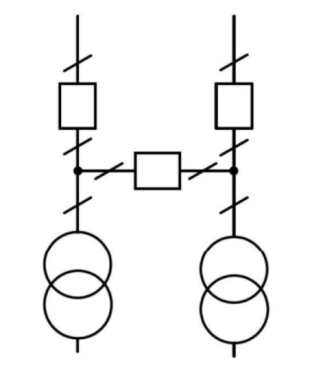
\includegraphics[width=0.2\textwidth]{inc/img/mostik}
	\caption{Схема РУ «мостик с выключателями в цепях линий»}
	\label{fig:мостик}
\end{figure}

\begin{figure}[ht]
	\centering
	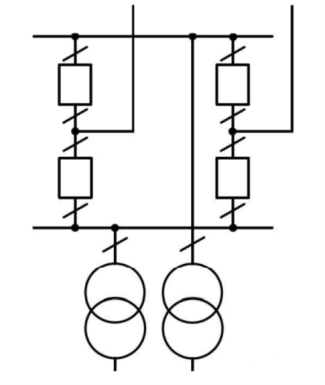
\includegraphics[width=0.2\textwidth]{inc/img/четырехугольник}
	\caption{Схема РУ «четырехугольник»}
	\label{fig:четырехугольник}
\end{figure}

\begin{figure}[ht]
	\centering
	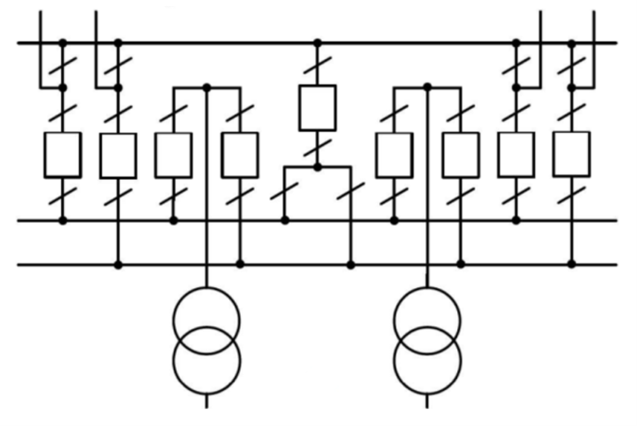
\includegraphics[width=0.4\textwidth]{inc/img/однорабоч_секц_с_обходкой}
	\caption{Схема РУ «одна рабочая секционированная выключателями и обходная системы шин с подключением трансформаторов к секциям шин через развилку из выключателей»}
	\label{fig:однарабоч_секц_с_обходкой}
\end{figure}

\begin{figure}[ht]
	\centering
	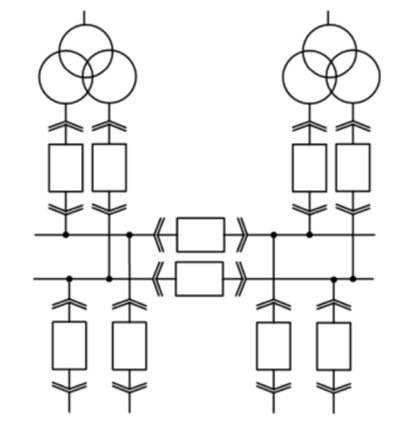
\includegraphics[width=0.3\textwidth]{inc/img/две_секц-ые_выключ}
	\caption{Схема РУ «две секционированные выключателями системы шин»}
	\label{fig:две_секц}
\end{figure}

\begin{figure}[ht]
	\centering
	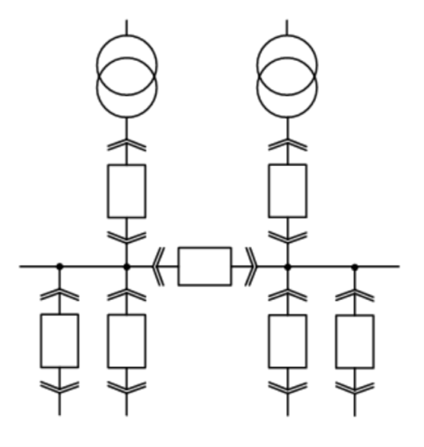
\includegraphics[width=0.3\textwidth]{inc/img/одна_секц-ая_выключ}
	\caption{Схема РУ «одна секционированная выключателем система шин»}
	\label{fig:одна_секц}
\end{figure}
\newpage

\section{Выбор схем РУ для варианта схемы сети 1}

\subsection*{Тупиковая ПС5 110/10}

На стороне ВН применяется схема «мостик с выключателями в цепях линий» (рис. \ref{fig:мостик}), так как ПС5 тупиковая, и к ней присоединяются две трёхфазные цепи линий. Количество ячеек выключателей 110 кВ РУ ВН равно \(n_\textup{яч5}^{110} = 3\).


На стороне НН применяется схема «две секционированные выключателями системы шин» (рис. \ref{fig:две_секц}), поскольку на ПС5 установлено два трансформатора ТРДН-25000/110 с расщепленной обмоткой НН. Суммарное количество ячеек в цепях силовых трансформаторов и секционных выключателей \(n_\textup{яч.тр.и.св5}^{10} = 6\). Всего на шинах НН ПС5 установлено 8 БСК (см. табл. \ref{tab:нагрузки_с_батареями_кольцо} и табл. \ref{tab:первичная_компенсация}), подключаемых к каждой секции через 4 выключателя, т.е. общее число выключателей компенсирующих устройств \(n_\textup{яч.пс5}^\textup{БСК}=4\). Количество линий 10 кВ, отходящих от шин НН понижающих подстанций, примерно оценивается исходя из нагрузки подстанции и мощности, условно приходящейся на одну линию 10 кВ – 3,5 МВА \cite{глазунов_шведов}:
\begin{eqndesc}[H]
	\[n_\textup{кл5}^\textup{1секц} = \frac{S_\textup{нб5}}{3,5\cdot n_\textup{секц5}} = \frac{38,5}{3,5 \cdot 4} = 2,75,\]
где \(n_\textup{кл5}^\textup{1секц}\)- число линий, отходящих от одной секции РУ НН ПС5; \(n_\textup{секц5}\) – число секций в выбранной схеме РУ НН ПС5.
\end{eqndesc}

Округляем полученное значение \(n_\textup{кл5}^\textup{1секц}\) до ближайшего целого числа. Получаем \(n_\textup{кл5}^\textup{1секц}\) = 3, следовательно, количество ячеек выключателей отходящих линий 10 кВ будет: \(n_\textup{кл5}^{10} = n_\textup{кл5}^\textup{1секц}\cdot n_\textup{секц5} = 3\cdot 4 = 12\)

Итого получим суммарное количество ячеек выключателей 10 кВ РУ НН:
\[n_\textup{яч5}^{10} = n_\textup{яч.тр.и.св5}^{10} + n_\textup{яч.пс5}^\textup{БСК} + n_\textup{кл5}^{10} = 6 + 4 + 12 = 22\]

\subsection*{Проходные ПС1 и ПС2 220/10}

На стороне ВН применяется схема «четырехугольник» (рис. \ref{fig:четырехугольник}), так как ПС1 и ПС2 проходные и имеют 4 подключения со стороны ВН. Количество ячеек выключателей 220 кВ РУ ВН равно \(n_\textup{яч1}^{220} = 4\).

На стороне НН применяется схема «две секционированные выключателями системы шин» (рис. \ref{fig:две_секц}), поскольку на ПС1 и ПС2 установлено два трансформатора ТРДН-63000/220 с расщепленной обмоткой НН. Суммарное количество ячеек в цепях силовых трансформаторов и секционных выключателей \(n_\textup{яч.тр.и.св1}^{10} = 6\). Всего на шинах НН ПС1 и ПС2 установлено 8 БСК (см. табл. \ref{tab:нагрузки_с_батареями_кольцо} и табл. \ref{tab:первичная_компенсация}), подключаемых к каждой секции через 4 выключателя, т.е. общее число выключателей компенсирующих устройств \(n_\textup{яч.пс1}^\textup{БСК}=4\). Количество линий 10 кВ, отходящих от шин НН понижающих подстанций:
\[n_\textup{кл1}^\textup{1секц} = \frac{S_\textup{нб1}}{3,5\cdot n_\textup{секц1}} = \frac{76,1}{3,5 \cdot 4} = 5,43\]

Округляем полученное значение \(n_\textup{кл1}^\textup{1секц}\) до ближайшего целого числа. Получаем \(n_\textup{кл1}^\textup{1секц}\) = 5, следовательно, количество ячеек выключателей отходящих линий 10 кВ будет: \(n_\textup{кл1}^{10} = n_\textup{кл1}^\textup{1секц}\cdot n_\textup{секц1} = 5\cdot 4 = 20\)

Итого получим суммарное количество ячеек выключателей 10 кВ РУ НН:
\[n_\textup{яч1}^{10} = n_\textup{яч.тр.и.св1}^{10} + n_\textup{яч.пс1}^\textup{БСК} + n_\textup{кл1}^{10} = 6 + 4 + 20 = 30\]

\subsection*{Проходная ПС4 110/10}

На стороне ВН применяется схема «одна рабочая секционированная выключателями и обходная системы шин с подключением трансформаторов к секциям шин через развилку из выключателей» (рис. \ref{fig:однарабоч_секц_с_обходкой}), так как ПС4 проходная, и к ней присоединяются 2 двухцепные трёхфазные цепи линий. Количество ячеек выключателей 110 кВ РУ ВН равно \(n_\textup{яч4}^{110} = 9\).

На стороне НН применяется схема «две секционированные выключателями системы шин» (рис. \ref{fig:две_секц}), поскольку на ПС4 установлено два трансформатора ТРДН-40000/110 с расщепленной обмоткой НН. Суммарное количество ячеек в цепях силовых трансформаторов и секционных выключателей \(n_\textup{яч.тр.и.св4}^{10} = 6\). Всего на шинах НН ПС4 установлено 8 БСК (см. табл. \ref{tab:нагрузки_с_батареями_кольцо} и табл. \ref{tab:первичная_компенсация}), подключаемых к каждой секции через 4 выключателя, т.е. общее число выключателей компенсирующих устройств \(n_\textup{яч.пс4}^\textup{БСК}=4\). Количество линий 10 кВ, отходящих от шин НН понижающих подстанций:
\[n_\textup{кл1}^\textup{1секц} = \frac{S_\textup{нб1}}{3,5\cdot n_\textup{секц1}} = \frac{44,9}{3,5 \cdot 4} = 3,21\]

Округляем полученное значение \(n_\textup{кл4}^\textup{1секц}\) до ближайшего целого числа. Получаем \(n_\textup{кл4}^\textup{1секц}\) = 3, следовательно, количество ячеек выключателей отходящих линий 10 кВ будет: \(n_\textup{кл4}^{10} = n_\textup{кл4}^\textup{1секц}\cdot n_\textup{секц4} = 3\cdot 4 = 12\)

Итого получим суммарное количество ячеек выключателей 10 кВ РУ НН:
\[n_\textup{яч4}^{10} = n_\textup{яч.тр.и.св4}^{10} + n_\textup{яч.пс4}^\textup{БСК} + n_\textup{кл4}^{10} = 6 + 4 + 12 = 22\]

\subsection*{Автотрансформаторная ПС3 220/110/10}

На стороне ВН применяется схема «четырехугольник» (рис. \ref{fig:четырехугольник}), так как ПС3 проходная и к ней присоединяются две трехфазные цепи: \(n_\textup{яч3}^{220} = 4\).

На стороне СН применяется схема «одна рабочая секционированная выключателями и обходная система шин с подключением трансформаторов к секциям шин через развилку из выключателей» (рис. \ref{fig:однарабоч_секц_с_обходкой}). Общее количество присоединенных цепей линий – 2 (двухцепная линия 3-4).

Количество ячеек выключателей 110 кВ РУ CН складывается из 1 ячейки для обходной системы шин, из 2 ячеек на каждое присоединение автотрансформатора и 1 ячейки на каждую отходящую трёхфазную цепь. С учётом того, что подключается 2 автотрансформатора и 2 цепи линий, получаем 7 ячеек: \(n_\textup{яч3}^{110} = 1 + 4 + 2 = 7\)

На стороне НН применяется схема «одна секционированная выключателем система шин» (рис. \ref{fig:одна_секц}). Суммарное количество ячеек в цепях силовых трансформаторов и секционных выключателей \(n_\textup{яч.тр.и.св3}^{10}=3\), поскольку на ПС установлены автотрансформаторы, где отсутствует расщепление обмотки НН. Всего на шинах НН ПС3 установлено 4 компенсирующих устройства, равномерно распределим их, по 2 на каждую секцию, и тогда число выключателей компенсирующих устройств \(n_\textup{яч3}^\textup{БСК}=2\). Количество ячеек выключателей отходящих линий 10 кВ будет:
\[n_\textup{кл3}^\textup{1секц}=S_\textup{нб3}/(3,5\cdot n_\textup{секц1} )=\frac{33,0}{3,5\cdot 2}= 4,71\]

Округляем полученное значение \(n_\textup{кл3}^\textup{1секц}\) до ближайшего целого числа. Получаем  \(n_\textup{кл3}^\textup{1секц} = 5\), следовательно, количество ячеек выключателей отходящих линий 10 кВ:
\[n_\textup{кл3}^{10}=n_\textup{кл3}^\textup{1секц}\cdot n_\textup{секц1} = 5 \cdot 2 = 10\]

Итого получим суммарное количество ячеек выключателей 10 кВ РУ НН:
\[n_\textup{яч3}^\textup{10} = 3 + 2 + 10 = 15\]

Результаты расчетов числа ячеек выключателей РУ разных классов номинального напряжения для обоих вариантов схемы сети сведены в табл. \ref{tab:параметры_ру_схема_1} и \ref{tab:параметры_ру_схема_2}.

\begin{table}[h]
	\small
	\caption{Параметры РУ для варианта схемы сети 1}
	\label{tab:параметры_ру_схема_1}
	\begin{tabularx}{\linewidth}{|l|Z|Z|Z|Z|Z|Z|}
		\hline
		ПС         & 3(АТ)  & 1 & 2 & 4 & 5 & \multirow{4}{*}{ИТОГО:} \\ \cline{1-6}
		Схема РУВН & рис. \ref{fig:четырехугольник} & рис. \ref{fig:четырехугольник}  & рис. \ref{fig:четырехугольник} & рис. \ref{fig:однарабоч_секц_с_обходкой} & \ref{fig:мостик} & \\ \cline{1-6}
		Схема РУСН & рис. \ref{fig:однарабоч_секц_с_обходкой} & - & - & - & - & \\ \cline{1-6}
		Схема РУНН & рис. \ref{fig:одна_секц} & рис. \ref{fig:две_секц} & рис. \ref{fig:две_секц} & рис. \ref{fig:две_секц} & рис. \ref{fig:две_секц} & \\ \hline
		\(n_\textup{яч}^{220}\) & 4 & 4 & 4 & - & - & 12 \\ \hline
		\(n_\textup{яч}^{110}\) & 7 & - & - & 9 & 3 & 19 \\ \hline
		\(n_\textup{яч.тр.и.св}^{10}\) & 3 & 6 & 6 & 6 & 6 & \multirow{8}{*}{} \\ \cline{1-6}
		\(N_\textup{БСК}\) & 4 & 8 & 8 & 8 & 8 & \\ \cline{1-6}
		\(n_\textup{яч}^\textup{БСК}\) & 2 & 4 & 4 & 4 & 4 & \\ \cline{1-6}
		\(S_\textup{нб}\), МВА & 33,0 & 76,1 & 76,1 & 44,9 & 38,5 & \\ \cline{1-6}
		\(S_\textup{нб} / (3,5\cdot n_\textup{секц})\) & 4,71 & 5,43 & 5,43 & 3,21 & 2,75 & \\ \cline{1-6}
		\(n_\textup{кл}^\textup{1секц}\) & 5 & 5 & 5 & 3 & 3 & \\ \cline{1-6}
		Расщепление (секц.) & - (2) & + (4) & + (4) & + (4) & + (4) & \\ \cline{1-6}
		\(n_\textup{кл}^{10}\) & 10 & 20 & 20 & 12 & 12 & \\ \hline
		\(n_\textup{яч}^{10}\) & 15 & 30 & 30 & 22 & 22 & 119 \\ \hline
	\end{tabularx}
\end{table}

\begin{table}[H]
	\small
	\caption{Параметры РУ для варианта схемы сети 2}
	\label{tab:параметры_ру_схема_2}
	\begin{tabularx}{\linewidth}{|l|Z|Z|Z|Z|Z|Z|}
		\hline
		ПС         & 3(АТ)  & 1 & 2 & 4 & 5 & \multirow{4}{*}{ИТОГО:} \\ \cline{1-6}
		Схема РУВН & рис. \ref{fig:однарабоч_секц_с_обходкой} & рис. \ref{fig:однарабоч_секц_с_обходкой}  & рис. \ref{fig:мостик} & рис. \ref{fig:однарабоч_секц_с_обходкой} & \ref{fig:мостик} & \\ \cline{1-6}
		Схема РУСН & рис. \ref{fig:однарабоч_секц_с_обходкой} & - & - & - & - & \\ \cline{1-6}
		Схема РУНН & рис. \ref{fig:одна_секц} & рис. \ref{fig:две_секц} & рис. \ref{fig:две_секц} & рис. \ref{fig:две_секц} & рис. \ref{fig:две_секц} & \\ \hline
		\(n_\textup{яч}^{220}\) & 9 & 9 & - & - & - & 18 \\ \hline
		\(n_\textup{яч}^{110}\) & 9 & - & 3 & 9 & 3 & 24 \\ \hline
		\(n_\textup{яч.тр.и.св}^{10}\) & 3 & 6 & 6 & 6 & 6 & \multirow{8}{*}{} \\ \cline{1-6}
		\(N_\textup{БСК}\) & 10 & 10 & 4 & 10 & 6 & \\ \cline{1-6}
		\(n_\textup{яч}^\textup{БСК}\) & 2 & 4 & 4 & 4 & 4 & \\ \cline{1-6}
		\(S_\textup{нб}\), МВА & 33,0 & 76,1 & 76,1 & 44,9 & 38,5 & \\ \cline{1-6}
		\(S_\textup{нб} / (3,5\cdot n_\textup{секц})\) & 4,71 & 5,43 & 5,43 & 3,21 & 2,75 & \\ \cline{1-6}
		\(n_\textup{кл}^\textup{1секц}\) & 5 & 5 & 5 & 3 & 3 & \\ \cline{1-6}
		Расщепление (секц.) & - (2) & + (4) & + (4) & + (4) & + (4) & \\ \cline{1-6}
		\(n_\textup{кл}^{10}\) & 10 & 20 & 20 & 12 & 12 & \\ \hline
		\(n_\textup{яч}^{10}\) & 15 & 30 & 30 & 22 & 22 & 119 \\ \hline
	\end{tabularx}
\end{table}


%%% Local Variables:
%%% mode: latex
%%% TeX-master: "rpz"
%%% End: